\scanpage{65}
% top, lines 1–2
\[
\left\{\begin{aligned}
s_0&=a_{-1},\ s_1=a_{-1}+a_0,\ s_2=a_{-1}+a_0+a_1,\ldots,\ s_{n+1}=a_{-1}+a_0+\cdots+a_n\\
s_{i+1}&=\tau_i s_i\qquad0\le i\le n
\end{aligned}\right.
\]

% upper, lines 3–4
\[
\left\{\begin{aligned}
s'_{n+1}&=a'_{n+1},\ s'_n=a'_{n+1}\unsure{-|+}a'_n,\ s'_{n-1}=a'_{n+1}+a'_n+a'_{n-1},\ldots,\ s'_0=a'_{n+1}+a'_n+\cdots+a'_0\\
s'_i&=\tau_i s'_{i+1}\qquad0\le i\le n.
\end{aligned}\right.
\]

% upper middle, lines 5–7
\[
\begin{aligned}
\langle s_i,\pi'\rangle&=1&\langle s_i,s'_j\rangle&=\begin{cases}0&\text{si }\deleted{j>i}\quad0\le i<j\le n+1\\1&\text{si }i=j,\quad0\le i\le n+1\end{cases}\\
\langle\pi,s'_i\rangle&=1\\
&&\langle s_i,\pi'\rangle&=1\qquad\langle\pi,s'_{\unsure{j|i}}\rangle=1\qquad0\le i\le n+1
\end{aligned}
\]

% above tᵢ group
\figure{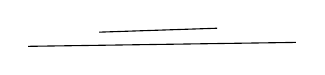
\begin{tikzpicture}\draw (0,0)--(3.4,.05);\draw (.9,.18)--(2.4,.23);\end{tikzpicture}}

% middle, lines 8–14
\[
\left\{\begin{aligned}
t_{\deleted{\unsure{n-}}i}&=\Theta(s'_i)\qquad0\le i\le n+1\\
\langle t_i,\pi\rangle&=-\beta\\
t_i&=\tau_i t_{i+1}\qquad0\le i\le n\\
&\boxed{\begin{aligned}
t_{n+1}=\Theta(s'_{n+1})&=-\sigma a_n^{\prime *}+\gamma\pi=-\sigma a_n^{\prime *}+\gamma a_{n+1}^{\prime *}\\
&=\gamma a_n+(2\gamma-\sigma)a_{n-1}+(\rho'_{n-1,n-1}\gamma-2\sigma)a_{n-2}+\cdots\\
&\quad+(\rho'_{n-1,n-1-j}\gamma\deleted{\unsure{_{n-j}}}-\rho'_{n-2,n-1-j}\sigma)a_{n-j-2}+\cdots\\
&\quad+(\rho'_{n-1,2}\deleted{\unsure{-}}\gamma-\rho'_{n-2,2}\sigma)a_1+\underset{!}{0\cdot a_0}\unsure{-|+}\beta a_{-1}
\end{aligned}}
\end{aligned}\right.
\]

% lower middle, lines 15–16
\[
\begin{aligned}
t_i&=t_{n+1}+\Theta(a'_n+\cdots+a'_i)\\
&=t_{n+1}-\sigma[a_n+\beta_{n-1}a_{n-1}+\beta_{n-1}\beta_{n-2}a_{n-2}+\cdots+(\beta_{n-1}\cdots\beta_i)a_i]
\end{aligned}
\]

% lower middle right, lines 15–16
\[
\Theta(a'_j)=-\sigma(\beta_{n-1}\cdots\beta_j)a_j\qquad0\le j\le n
\]

% lower, lines 17–19
\uline{NB} $t_i=0$ (pour $i$ fixé) sss $\sigma=\gamma=0$ (et \unsure{ceci|celà} implique $\beta=0$)

Si $\beta$ inv. (mais sans que néc. $\sigma$ inv. i.e. $\psi$ iso) alors

On peut définir $-\frac{1}{\beta}t_i\deleted{\unsure{a}}\in\unsure{E|\bar E}\subset X$ \ldots.

% foot, lines 20–22
\[
\begin{aligned}
\varphi(t_{n+1},s_i)&=0\qquad0\le i\le n&\varphi(t_{n+1},s_{n+1})&=\varphi(t_{n+1},a_n)=\beta\sigma\\
\varphi(t_{n+1},a_i)&=0\qquad-1\le i\le n-1\\
f(t_{n+1})&=\tfrac12\langle t_{n+1},\underbrace{\psi(t_{n+1})}_{\beta\sigma s'_{n+1}}\rangle=\frac{\beta\sigma}{2}\gamma=\beta\widetilde{\sigma}\widetilde{\gamma}
\end{aligned}
\]

% foot right, struck draft and replacement
\[
\begin{aligned}
&\deleted{\langle t_{n+1},\psi(a_n)\rangle=(-2\gamma+2\gamma-\sigma)(-\beta)\sigma}\\
&\deleted{=\beta a'_n\,\psi t_{n+1}}\quad\langle a_n,\underbrace{\psi(t_{n+1})}_{\beta\sigma s'_{n+1}}\rangle
\end{aligned}
\]

% foot, left
% archive sheet number: 64

